
\section{Designer diagnostics}\label{app:designer}
The annealing designer of the methods section optimizes the ensemble score
with a novelty floor. Table~\ref{tab:alldesigns} lists the top-10 anneals;
Figure~\ref{fig:anneal} shows the score--novelty plane. The anneals
cluster at novelty 0.89--0.96 against the training corpus: the novelty
floor is active, and the optimizer is not simply memorizing a training
motif. All designs are short (25--57 aa), cationic and hydrophobic by
construction of the scoring function; none is a claimed AMP, and each
carries the same training-label confound as the screen candidates
(Section~\ref{sec:labelconfound}).

\begin{figure}[h]\centering
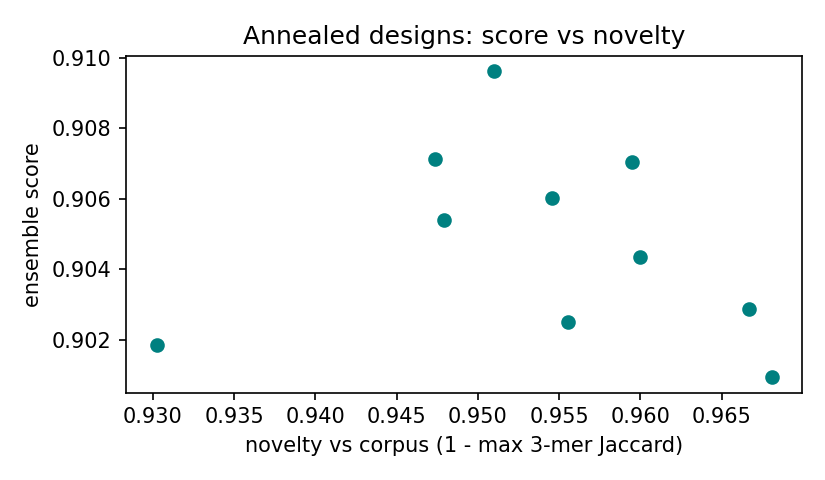
\includegraphics[width=0.65\textwidth]{fig_anneal.png}
\caption{Annealed designs in the score--novelty plane.}
\label{fig:anneal}
\end{figure}
